\begin{figure}[t]
  \centering
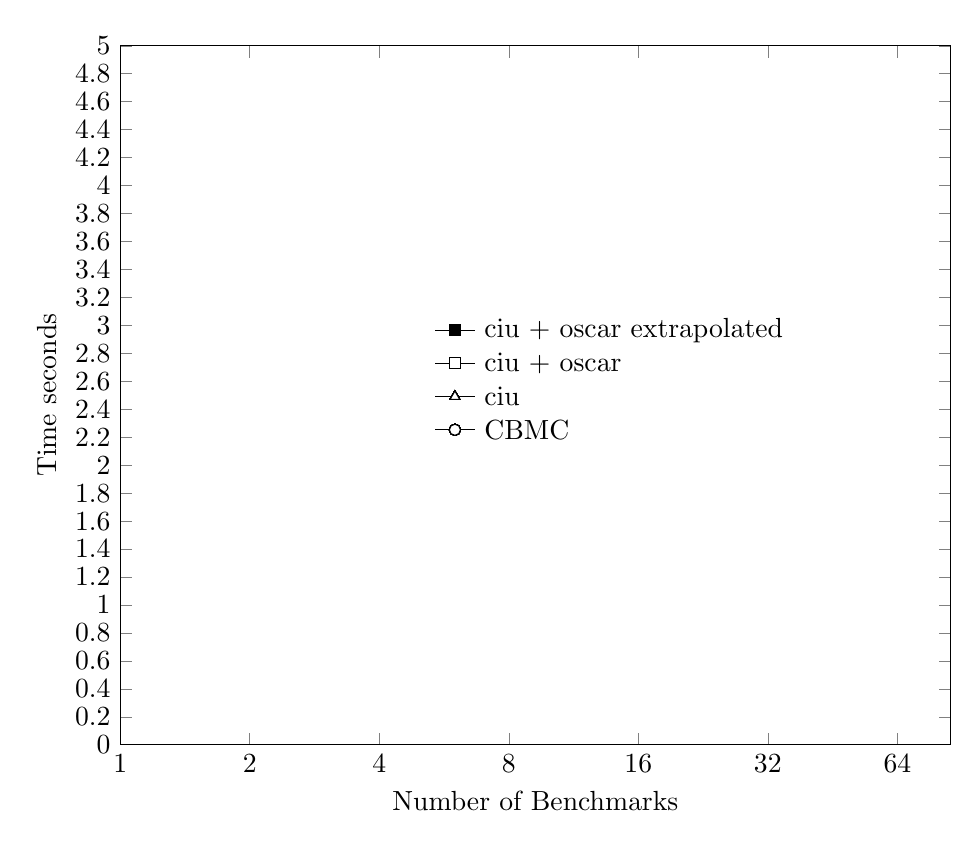
\begin{tikzpicture}
 	%axis
  \begin{axis}[
    width=\linewidth,
    xlabel={Number of Benchmarks},
    ylabel={Time seconds},
    domain = 1:85,
    xmin=1, xmax=85,
    ymin=0, ymax=5,
    ytick={0,0.2,0.4,...,5},
    xmode = log,
    log basis x={2},
    xticklabel=\pgfmathparse{2^\tick}\pgfmathprintnumber{\pgfmathresult},
    legend pos = north west
  ]
    %\addplot [dashed]
    % {plotdata/cbmc-time.dat};
	%plots
	\draw plot[mark=*, mark options={fill=white}] 
		file {plotdata/cbmc-time.dat};
	%\draw plot[mark=triangle*, mark options={fill=white} ] 
	%	file {div_ciu.dat};
	%\draw plot[mark=square*, mark options={fill=white}]
	%	file {div_ciu_oscar.dat};
	%\draw plot[mark=square*]
	%	file {div_ciu_oscar_extrapolated.dat};  
  \end{axis}  
	%legend
	\begin{scope}[shift={(4,4)}] 
	\draw (0,0) -- 
		plot[mark=*, mark options={fill=white}] (0.25,0) -- (0.5,0) 
		node[right]{CBMC};
    \Omit{
  \draw[yshift=\baselineskip] (0,0) -- 
		plot[mark=triangle*, mark options={fill=white}] (0.25,0) -- (0.5,0)
		node[right]{ciu};
	\draw[yshift=2\baselineskip] (0,0) -- 
		plot[mark=square*, mark options={fill=white}] (0.25,0) -- (0.5,0)
		node[right]{ciu + oscar};
	\draw[yshift=3\baselineskip] (0,0) -- 
		plot[mark=square*, mark options={fill=black}] (0.25,0) -- (0.5,0)
		node[right]{ciu + oscar extrapolated};
    }
  \end{scope}
\end{tikzpicture}
\caption{\label{fig:results}
  Runtime Comparison between CBMC, Astr{\'e}e and ACDLP}
\end{figure}
